\begin{subfigures}

	\begin{figure}[!htbp]
		{
			\renewcommand{\arraystretch}{0.1}
			\centering	
			%	\subfloat[]{
			\begin{tabular}{|p{.5cm} c c|}
				\hline
				&&\\[1em]
				&	\phewon\ 	& \simple \\[1.5em]
				%
				%
				\begin{sideways}{\hspace{3cm} \textbf{All particles}}\end{sideways} \hspace*{-1em}	&		 
				{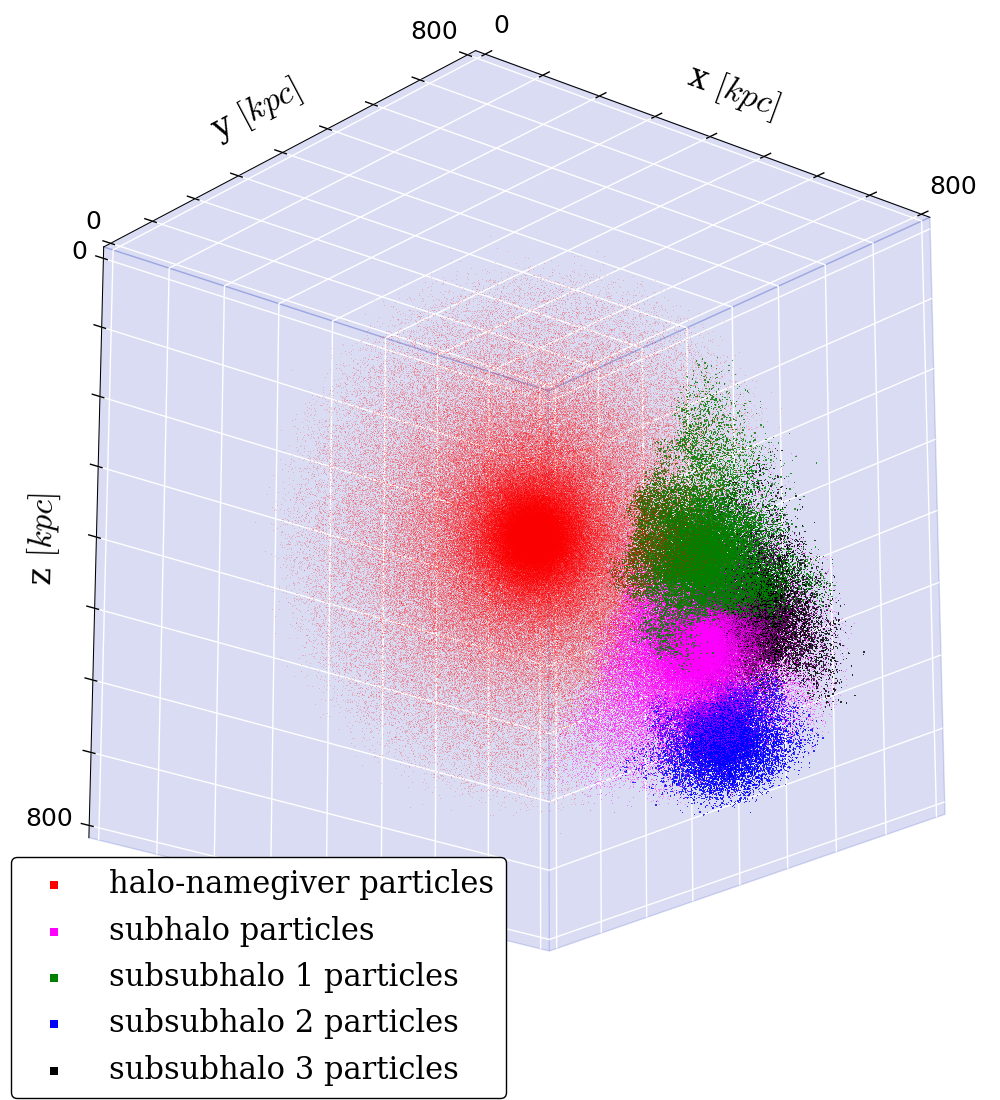
\includegraphics[width = .42\textwidth]{images/dice-sub/dice-sub-plot-halo1-phew.png}} \hspace*{-1em} 	& 
				{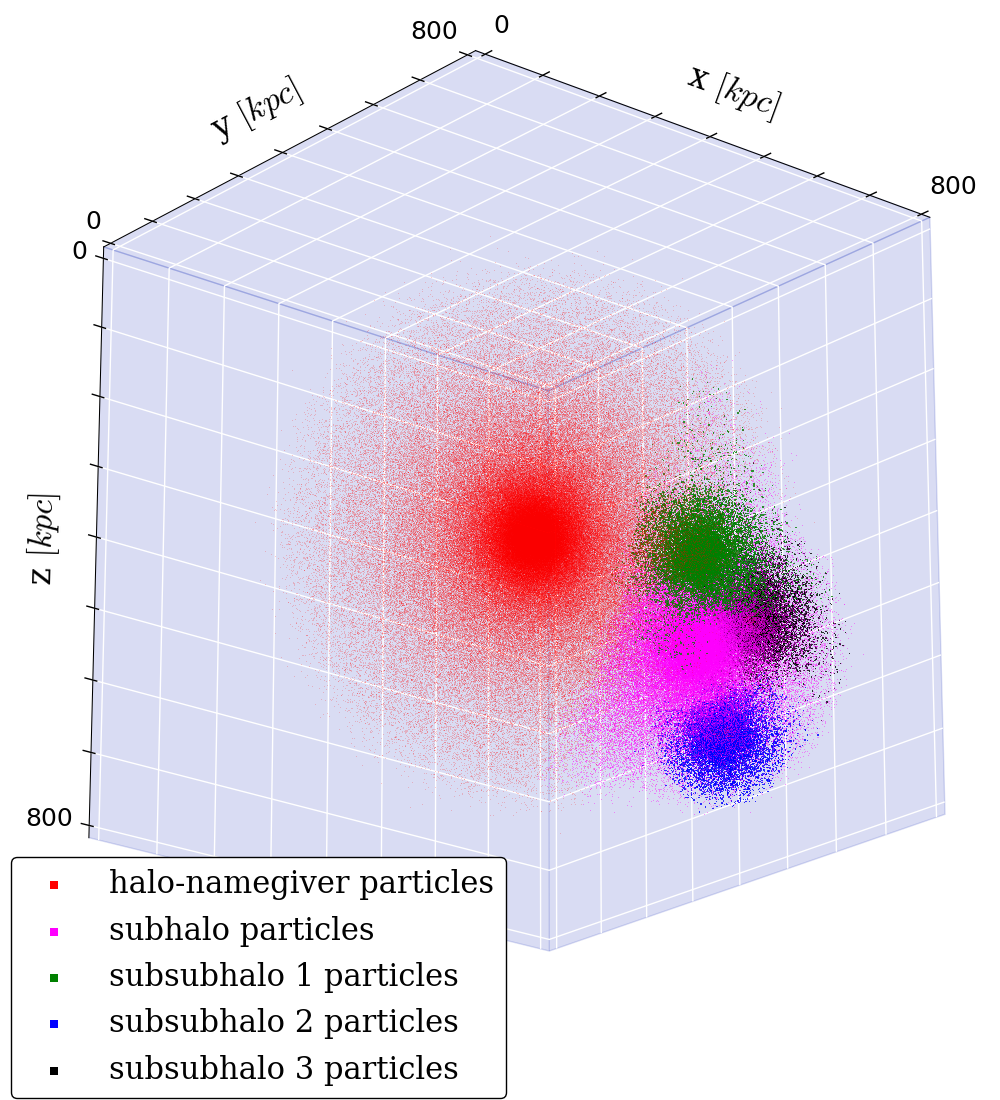
\includegraphics[width = .42\textwidth]{images/dice-sub/dice-sub-plot-halo1-nosaddle.png}} \hspace*{-1em}	\\
				%
				%
				\begin{sideways}{ \hspace{.5cm}\textbf{Halo-namegiver particles only} }\end{sideways}	 \hspace*{-1em}			 &			 
				{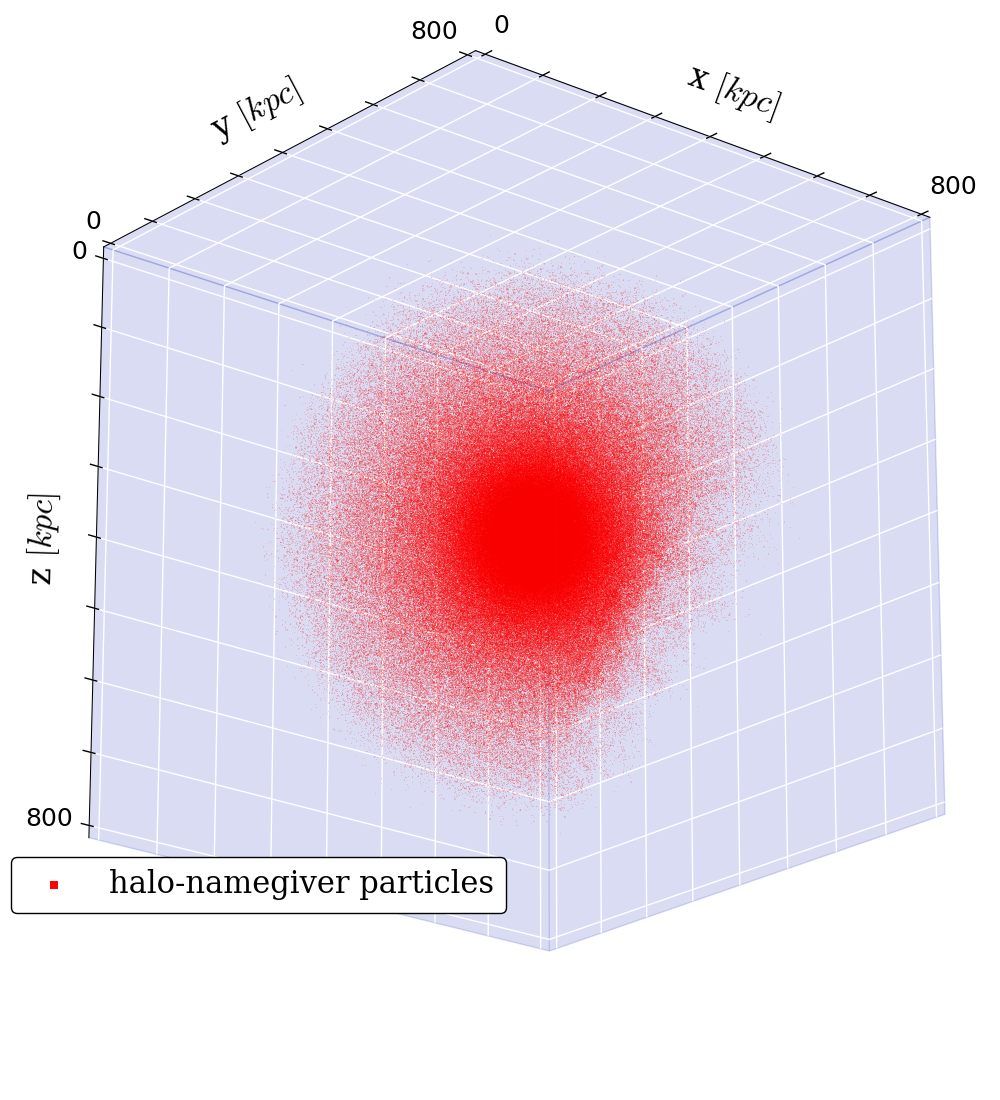
\includegraphics[width = .42\textwidth]{images/dice-sub/dice-sub-halo-only-phew.png}} \hspace*{-1em} 		&
				{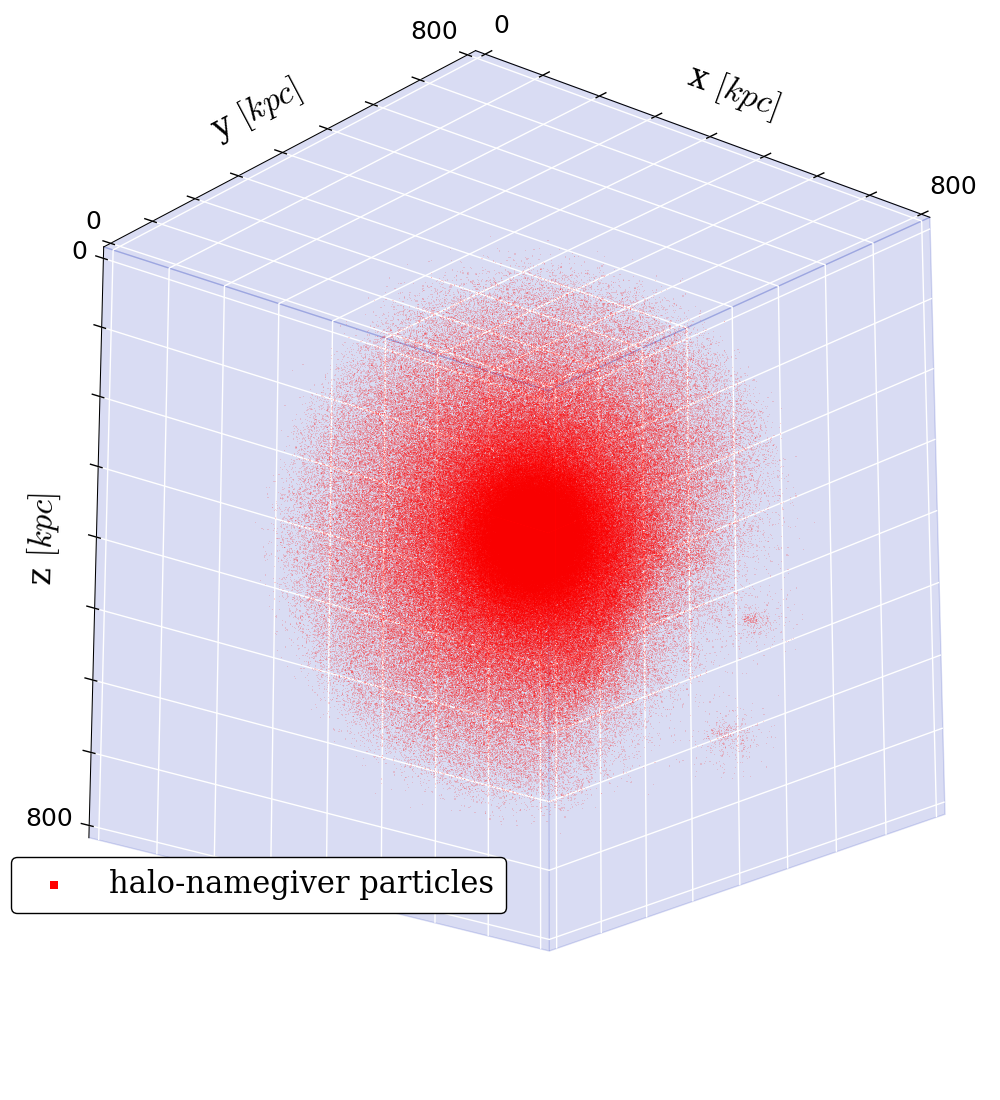
\includegraphics[width = .42\textwidth]{images/dice-sub/dice-sub-halo-only-nosaddle.png}} \hspace*{-1em}		\\
				%
				%
				\begin{sideways}{ \hspace{2cm}\textbf{Subhalo particles only} }\end{sideways}	 \hspace*{-1em}			 &
				{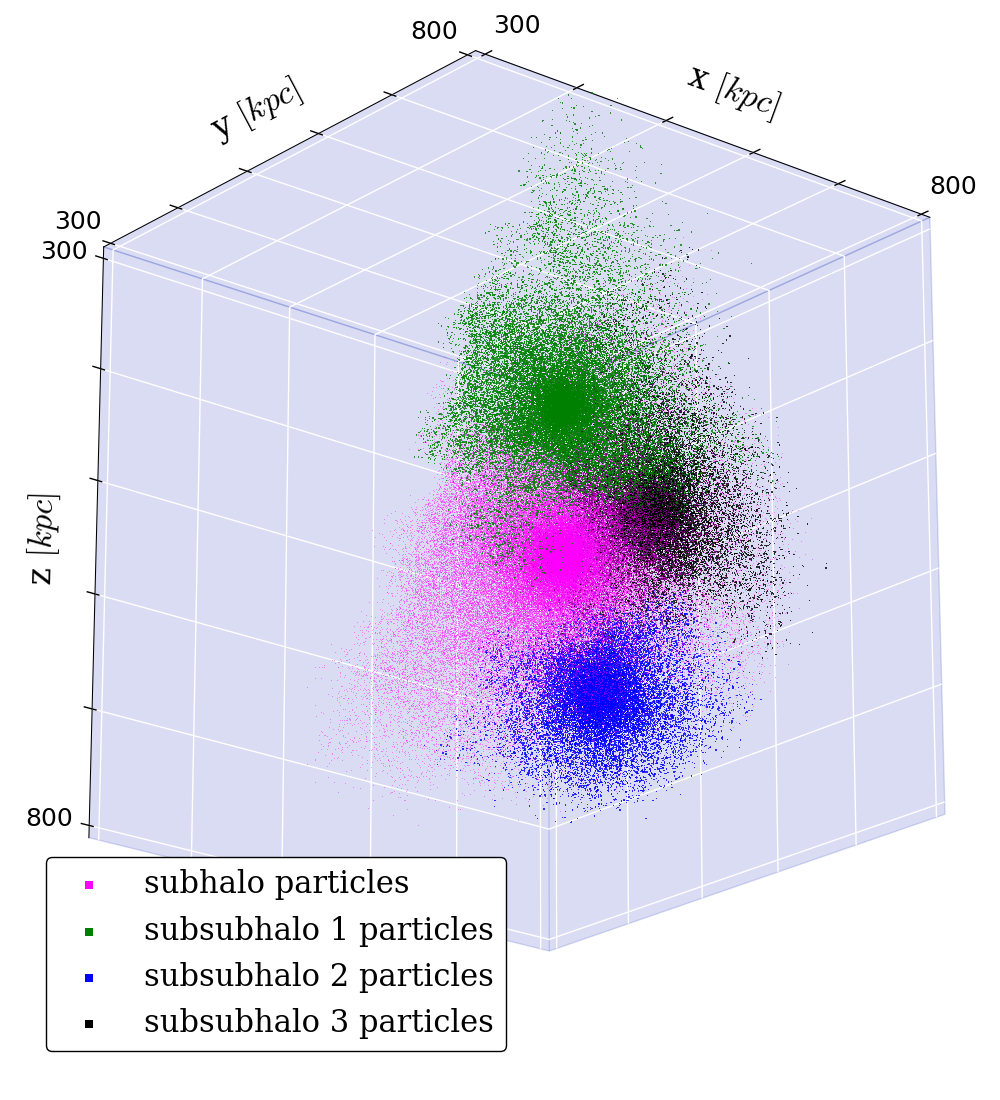
\includegraphics[width = .42\textwidth]{images/dice-sub/dice-sub-plot-subclumps-phew.png}} &
				{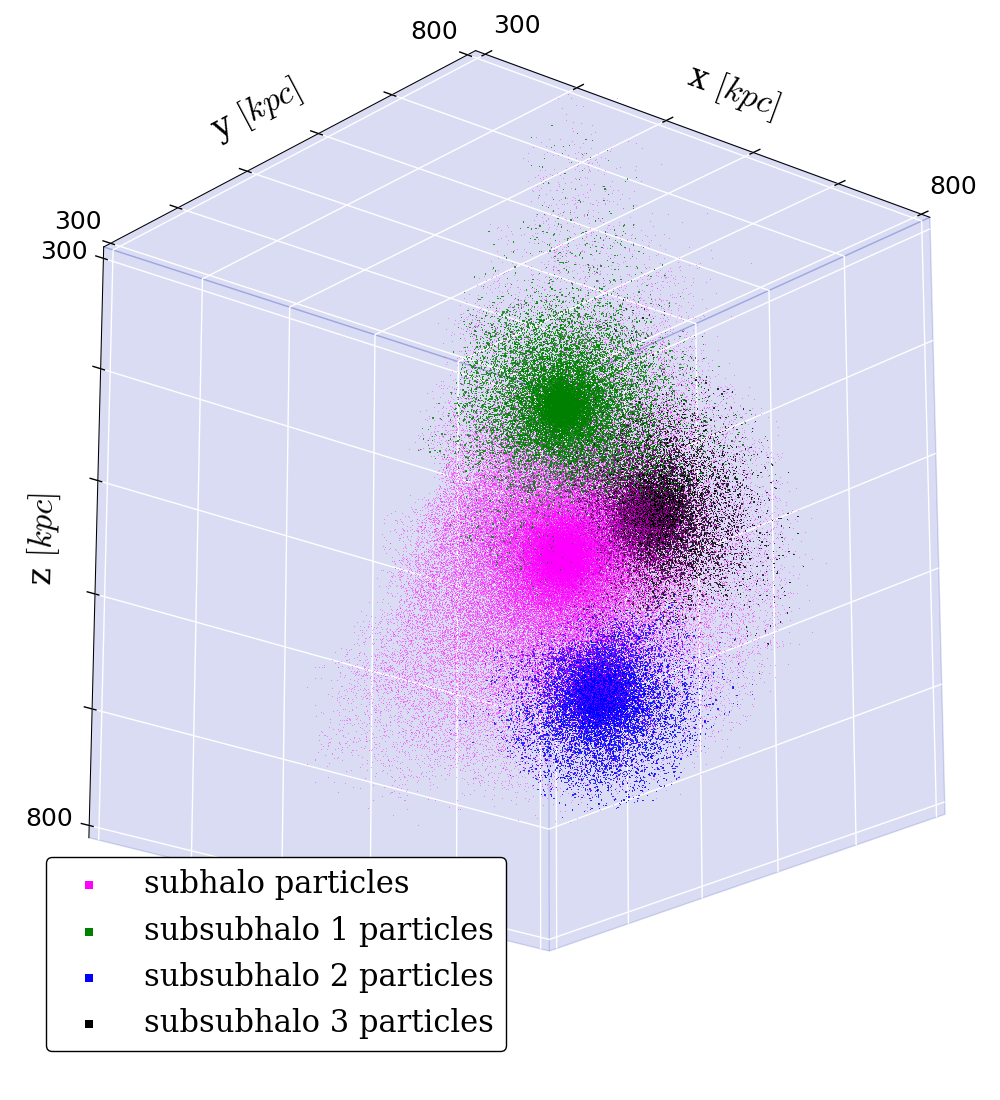
\includegraphics[width = .42\textwidth]{images/dice-sub/dice-sub-plot-subclumps-nosaddle.png}} \\
				\hline
			\end{tabular}
			\caption{\label{fig:dice_sub_results_a}The results of \phewon\ and \simple\ unbinding of the \ds-dataset: All particles, halo-namegiver particles only and subhalo particles only.}
		}
	\end{figure}
	%=================================================
	%=================================================
	%=================================================
	\begin{figure}[!htbp]%\ContinuedFloat
		{
			\renewcommand{\arraystretch}{0.1}
			\centering	
			\begin{tabular}{|p{.5cm} c c|}
				\hline
				&&\\[1em]
				&	\neigh\ 	& \iter \\[1.5em]
				%
				%
				\begin{sideways}{\hspace{3cm} \textbf{All particles}}\end{sideways} \hspace*{-1em}	&		 
				{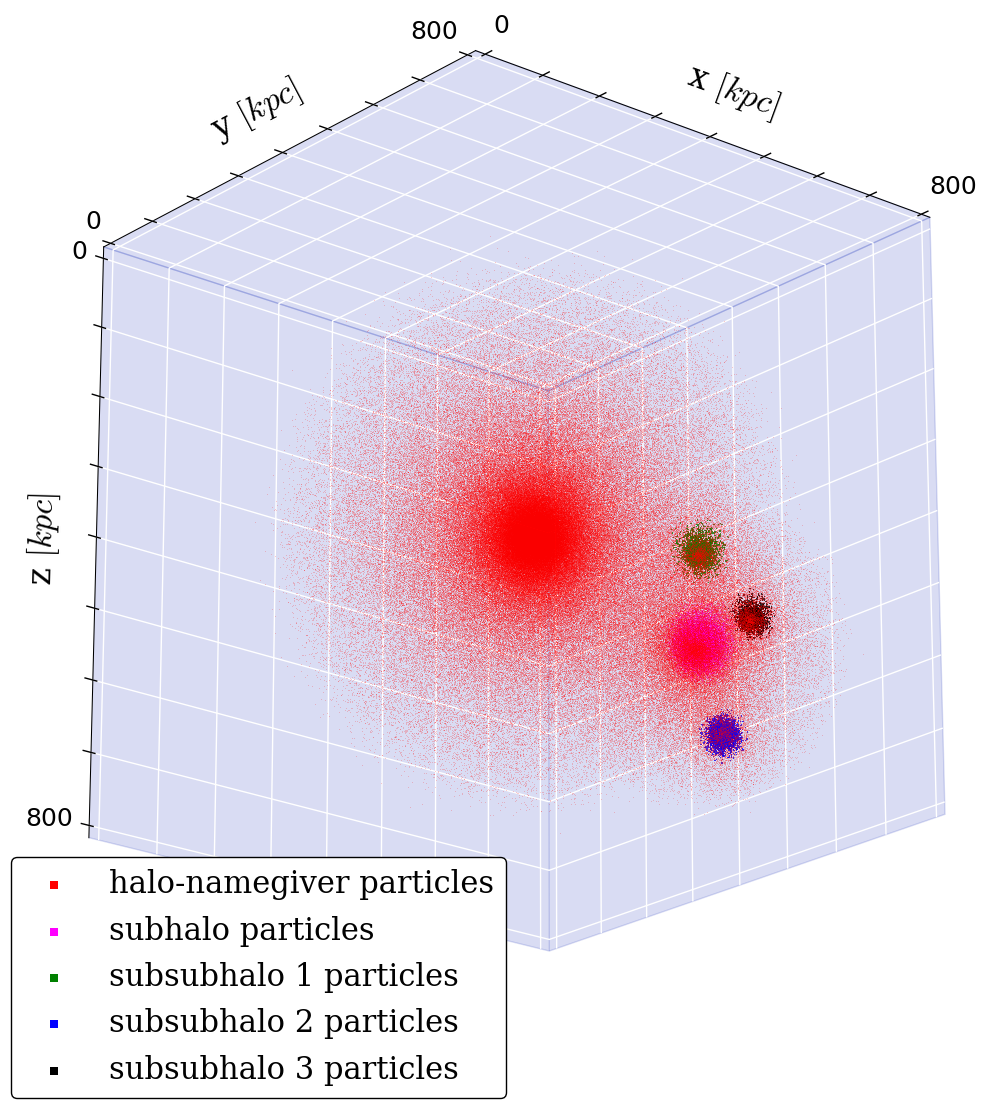
\includegraphics[width = .42\textwidth]{images/dice-sub/dice-sub-plot-halo1-saddle.png}} \hspace*{-1em} 	& 
				{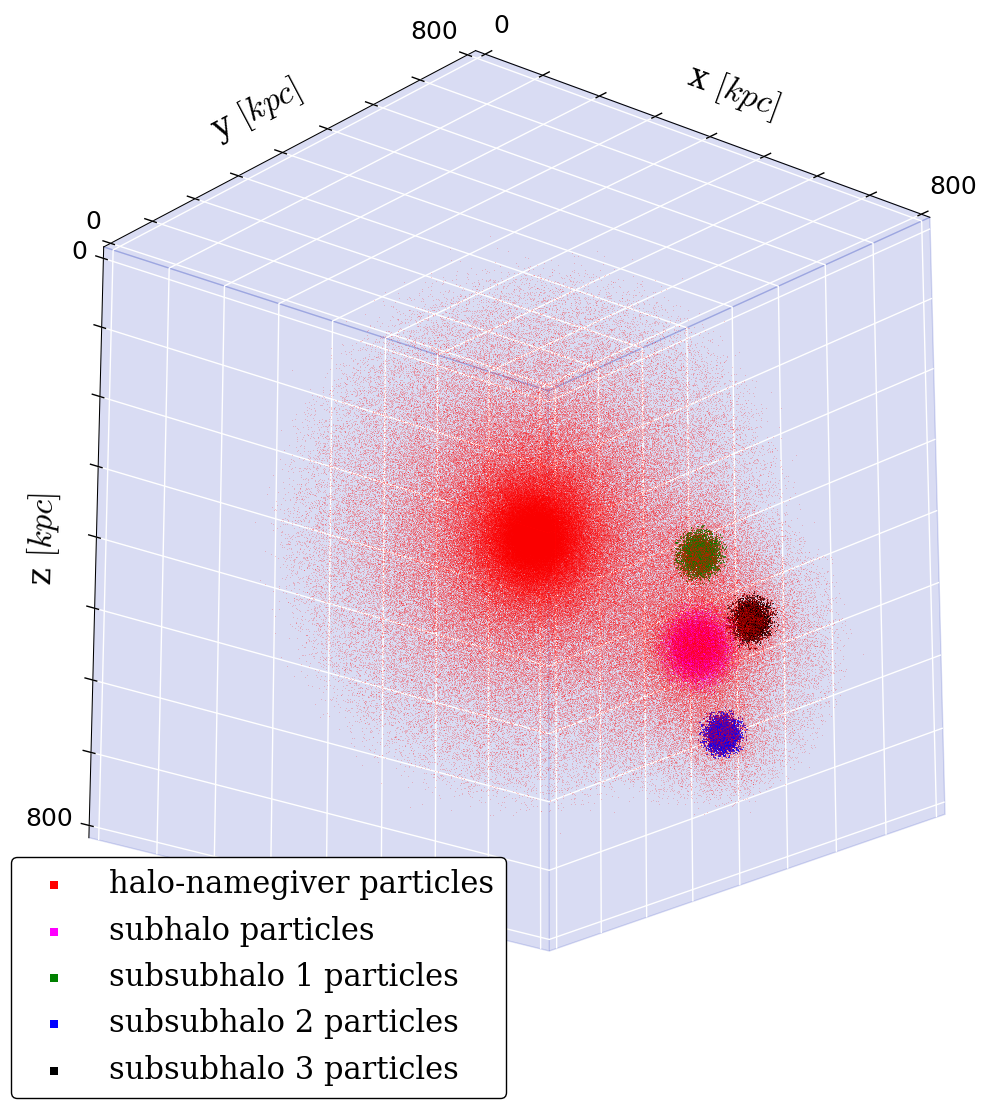
\includegraphics[width = .42\textwidth]{images/dice-sub/dice-sub-plot-halo1-iter.png}} \hspace*{-1em}	\\
				%
				%
				\begin{sideways}{ \hspace{.5cm}\textbf{Halo-namegiver particles only} }\end{sideways}	 \hspace*{-1em}			 &			 
				{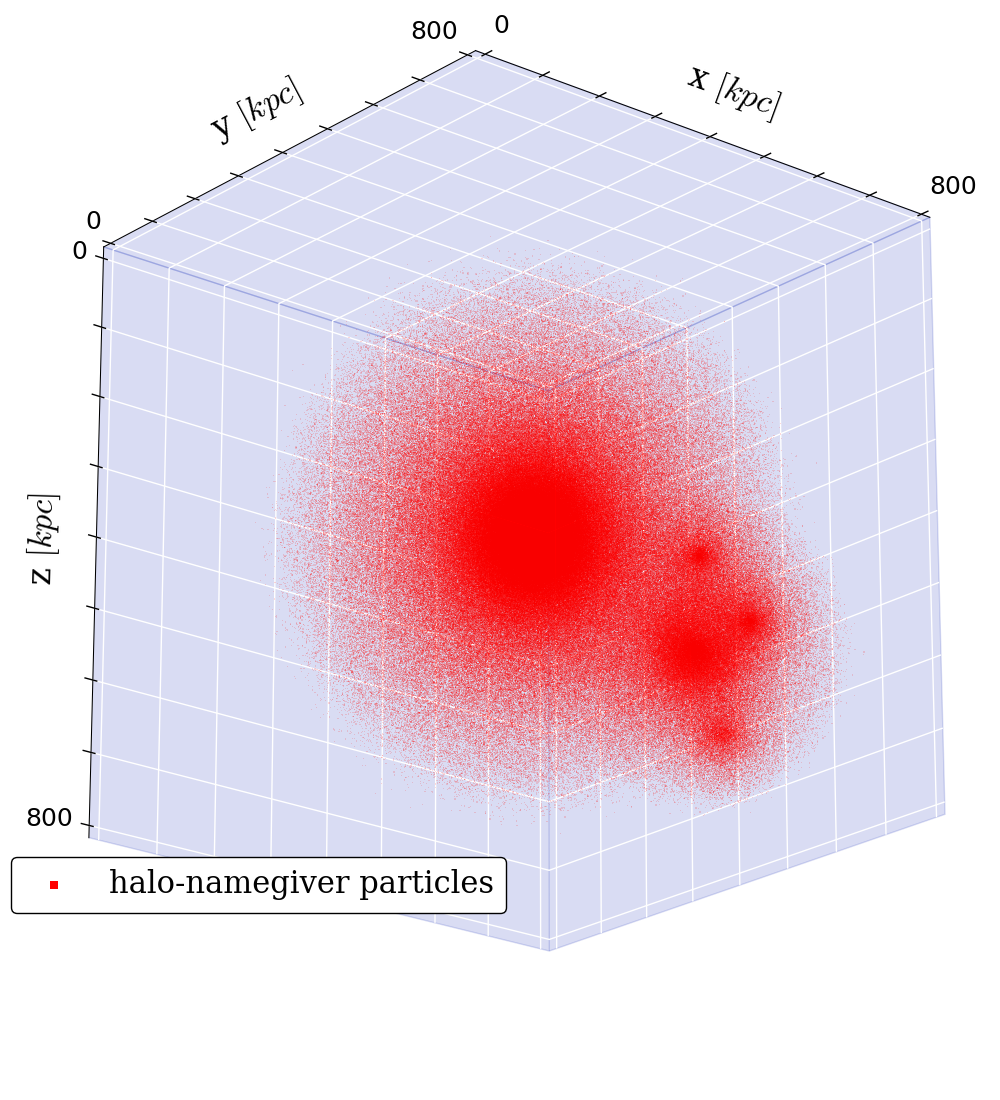
\includegraphics[width = .42\textwidth]{images/dice-sub/dice-sub-halo-only-saddle.png}} \hspace*{-1em} 		&
				{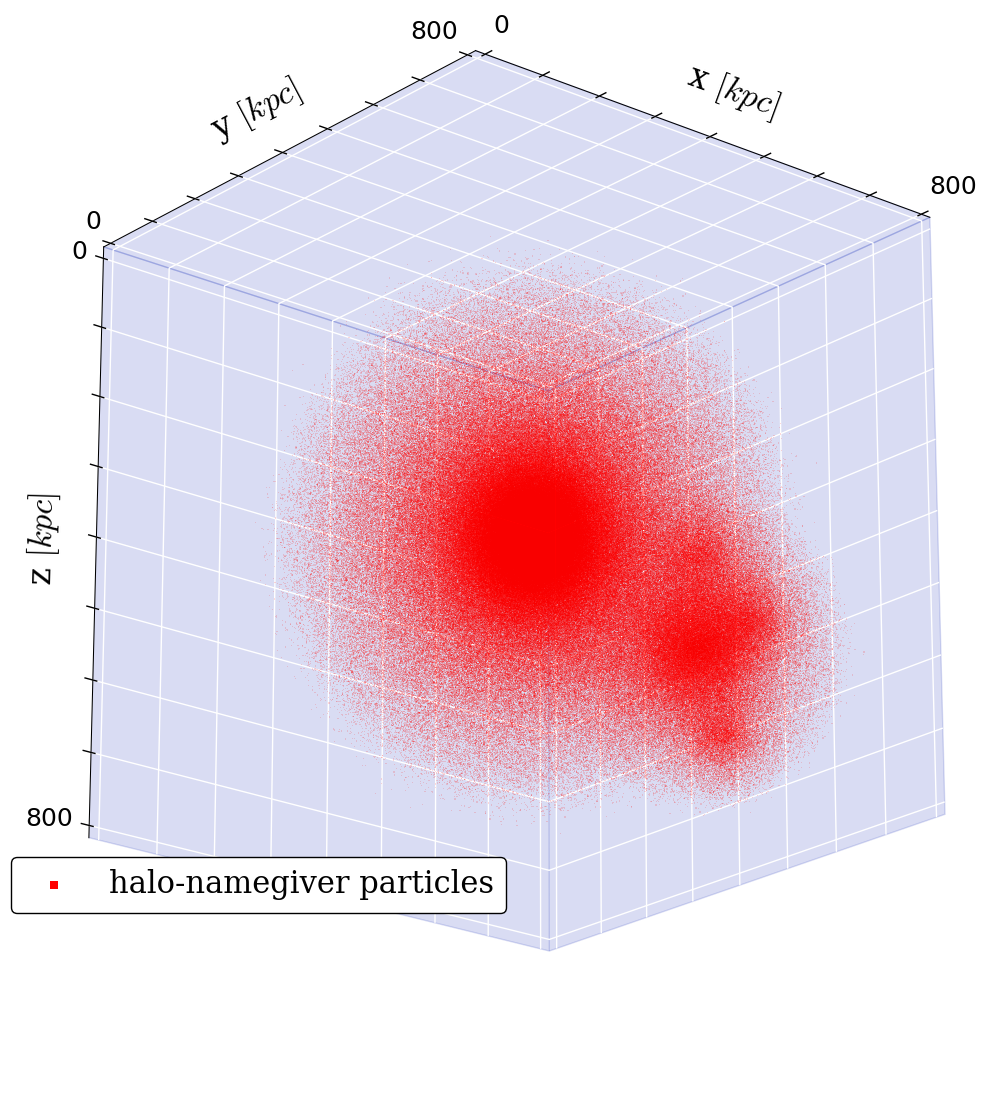
\includegraphics[width = .42\textwidth]{images/dice-sub/dice-sub-halo-only-iter.png}} \hspace*{-1em}		\\
				%
				%
				\begin{sideways}{ \hspace{2cm}\textbf{Subhalo particles only} }\end{sideways}	 \hspace*{-1em}			 &
				{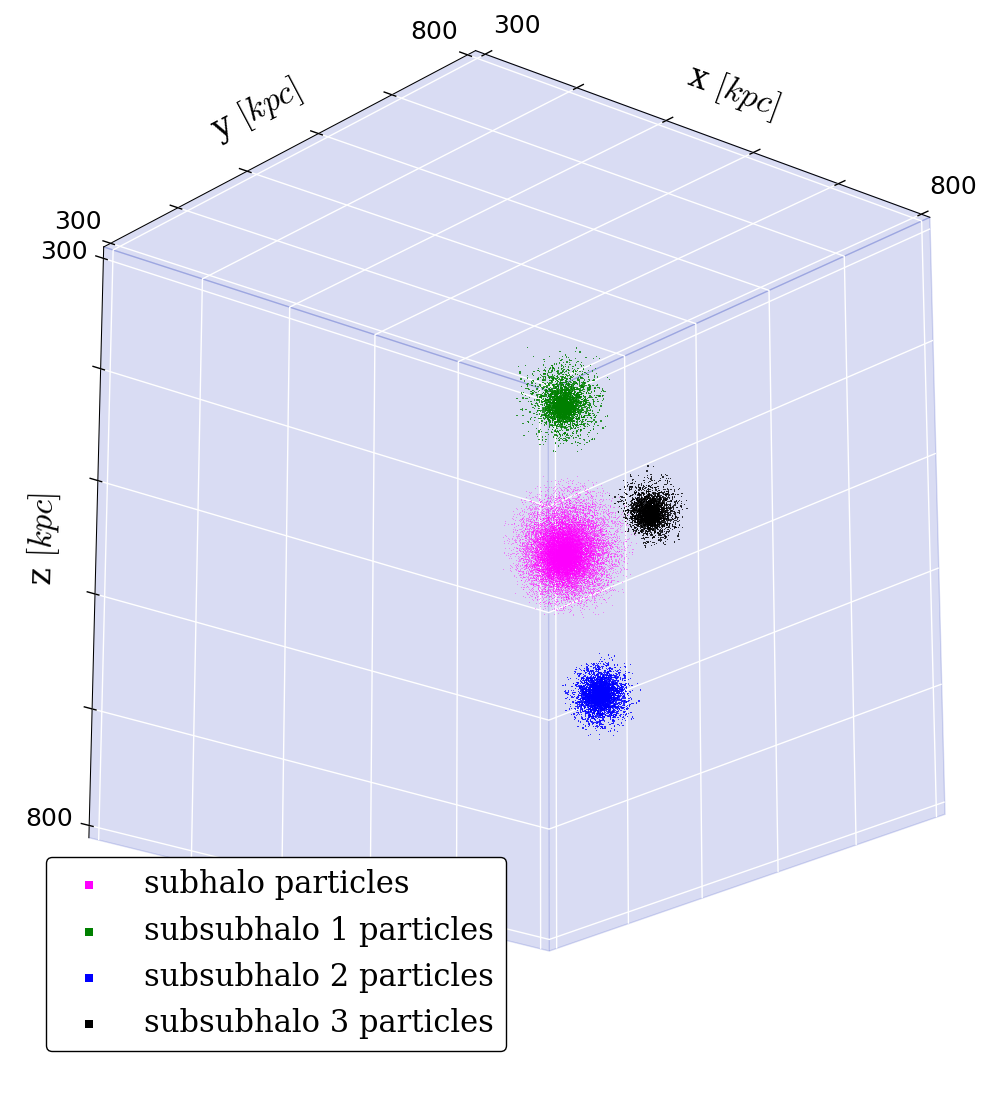
\includegraphics[width = .42\textwidth]{images/dice-sub/dice-sub-plot-subclumps-saddle.png}} &
				{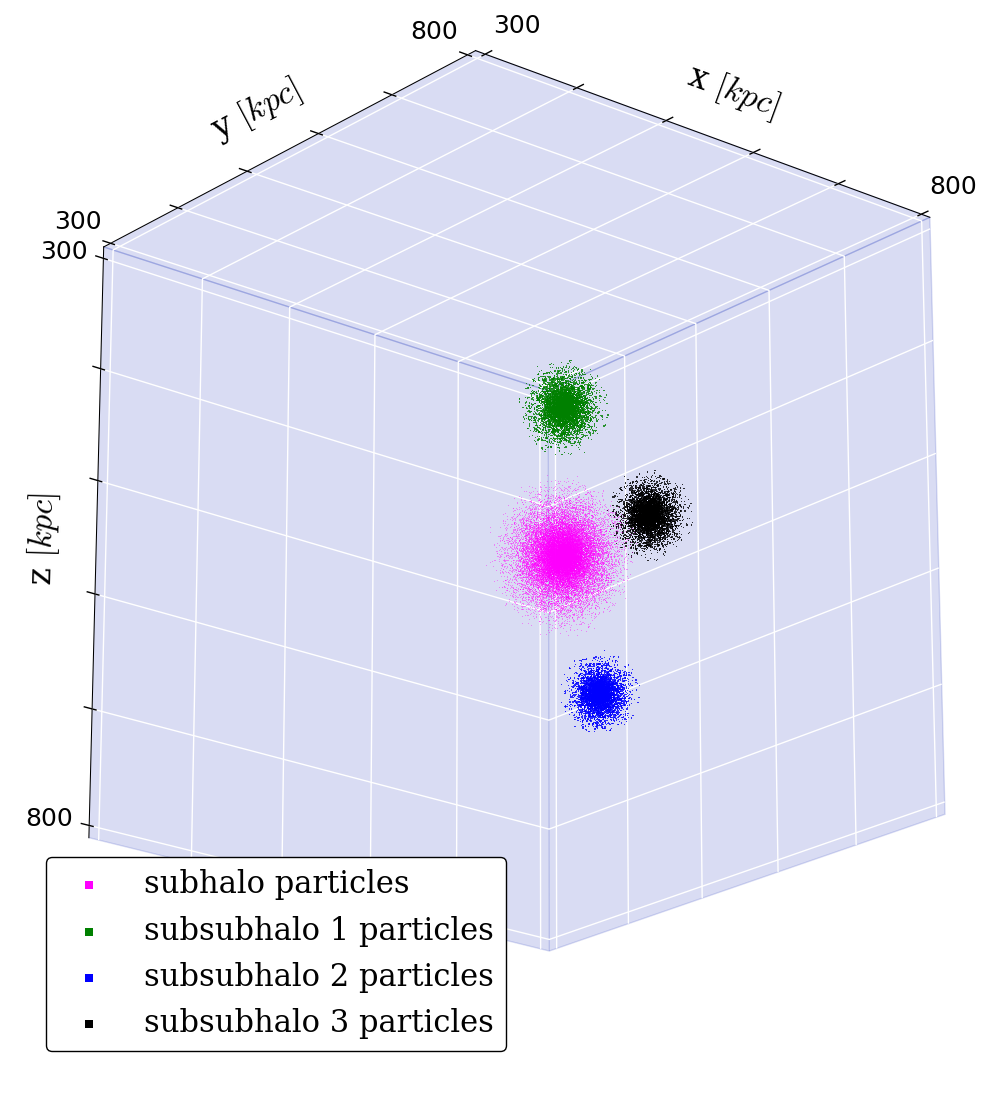
\includegraphics[width = .42\textwidth]{images/dice-sub/dice-sub-plot-subclumps-iter.png}} \\
				\hline
			\end{tabular}
			\caption{\label{fig:dice_sub_results_b}
				The results of \neigh\ and \iter\ unbinding of the \ds-dataset: All particles, halo-namegiver particles only and subhalo particles only.
			}
		}
	\end{figure}
	\label{fig:dice_sub_results}
\end{subfigures}




























































%\begin{sidewaysfigure}[!htbp]
%	{\renewcommand{\arraystretch}{0.1}
%		
%	\subfloat[The results of \phewon\ and \simple\ unbinding of the \ds-dataset: All particles, halo-namegiver particles only and subclumps particles only.]{
%		\begin{tabular}{|p{1cm} c c c|}
%			\hline
%			&&&\\[1em]
%													&
%			\textbf{All particles} 					&
%			\textbf{Halo-namegiver particles only} 	&
%			\textbf{Subhalo particles only} 		\\[1em]
%			%
%			%
%			\begin{sideways}{\hspace{3cm} \phewon}\end{sideways} \hspace*{-1em}%		 
%			& {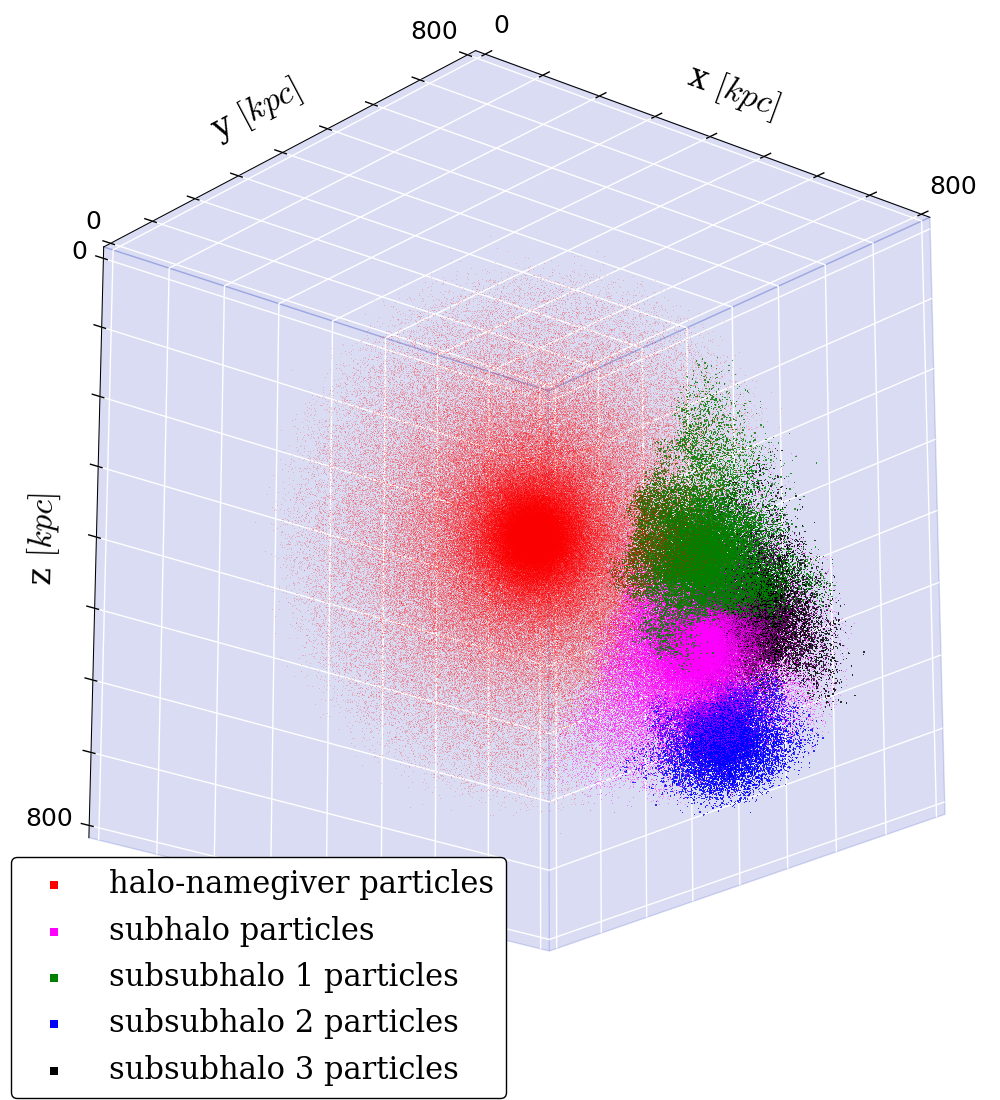
\includegraphics[width = .28\textwidth]{images/dice-sub/dice-sub-plot-halo1-phew.png}} \hspace*{-1em}%
%			 & {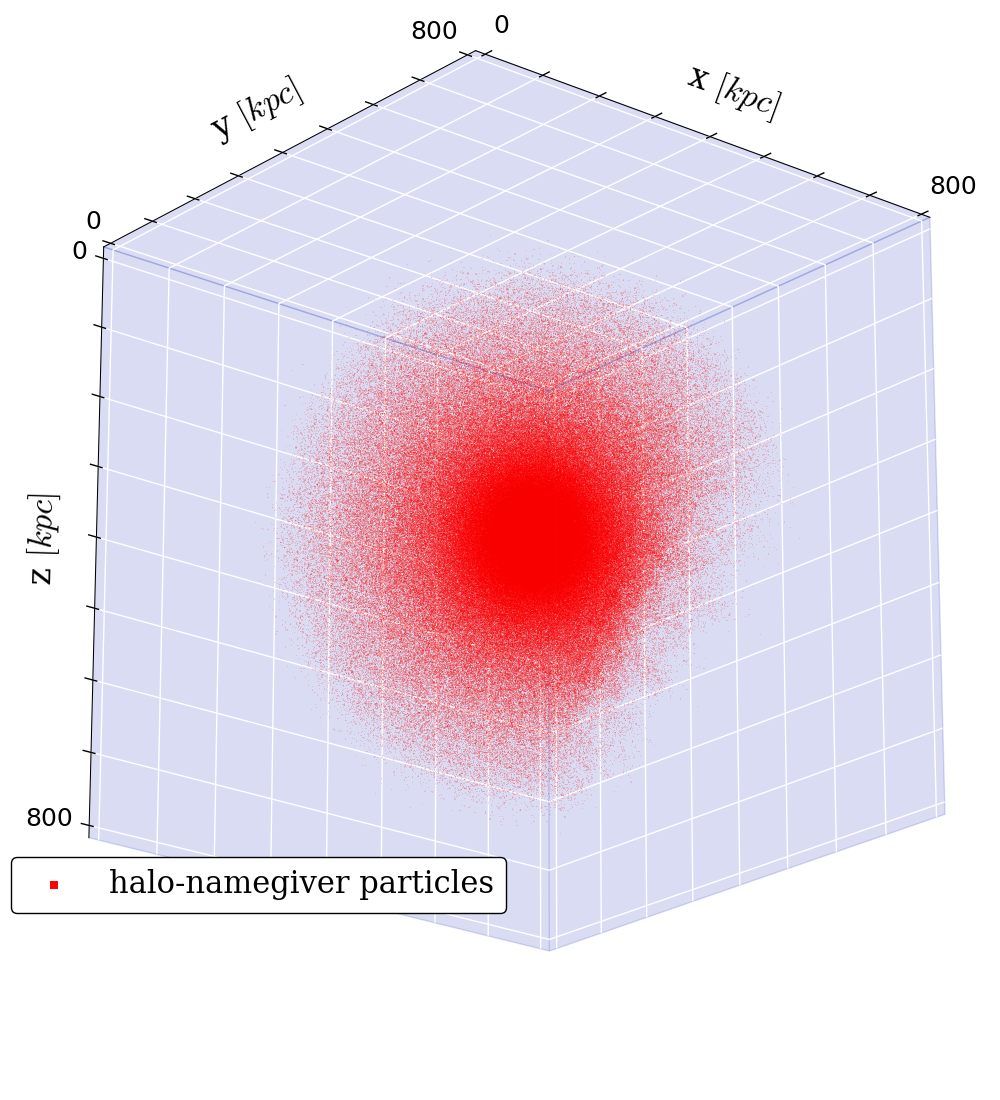
\includegraphics[width = .28\textwidth]{images/dice-sub/dice-sub-halo-only-phew.png}} \hspace*{-1em}% 
%			 &{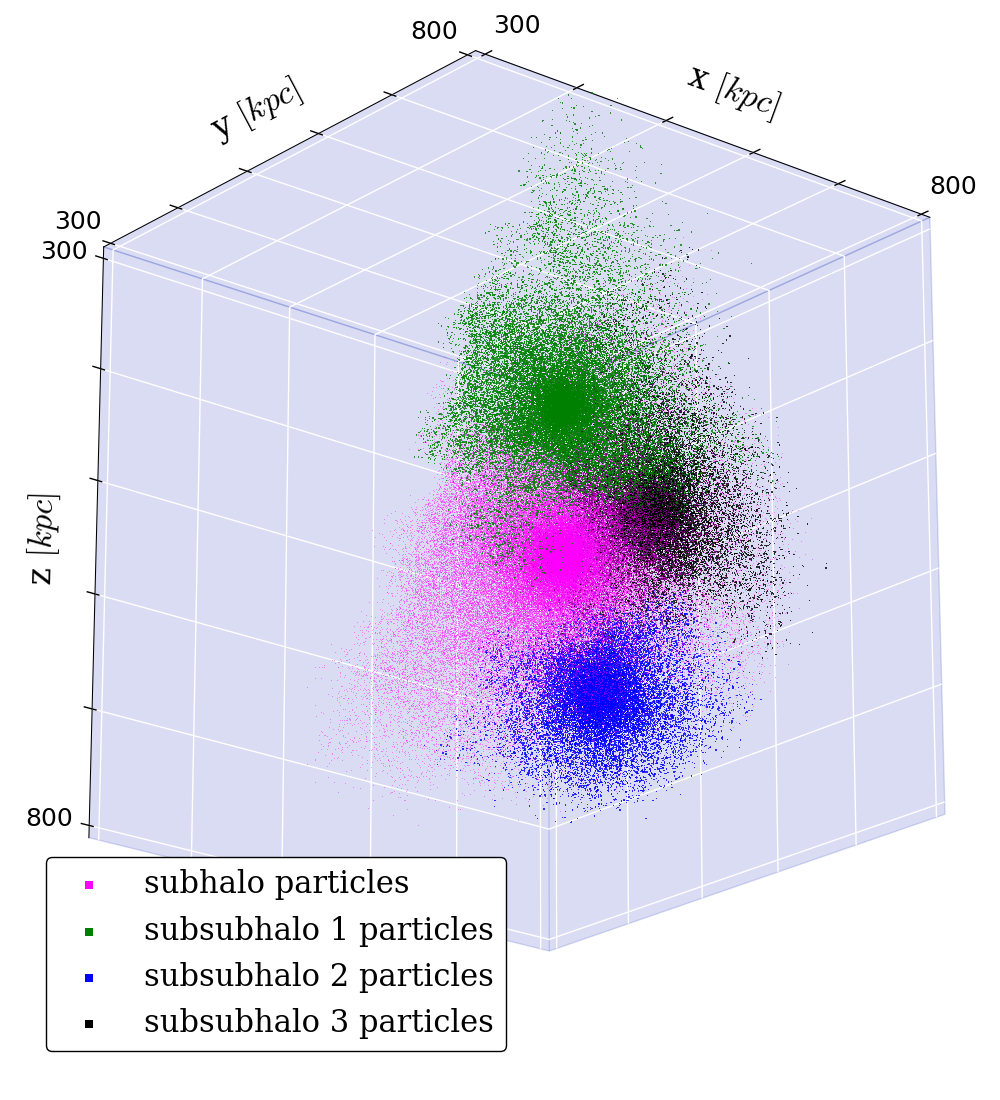
\includegraphics[width = .28\textwidth]{images/dice-sub/dice-sub-plot-subclumps-phew.png}} \\
%			%
%			%
%			\begin{sideways}{ \hspace{3cm}\simple\ unbinding }\end{sideways}	 \hspace*{-1em}			 &
%			{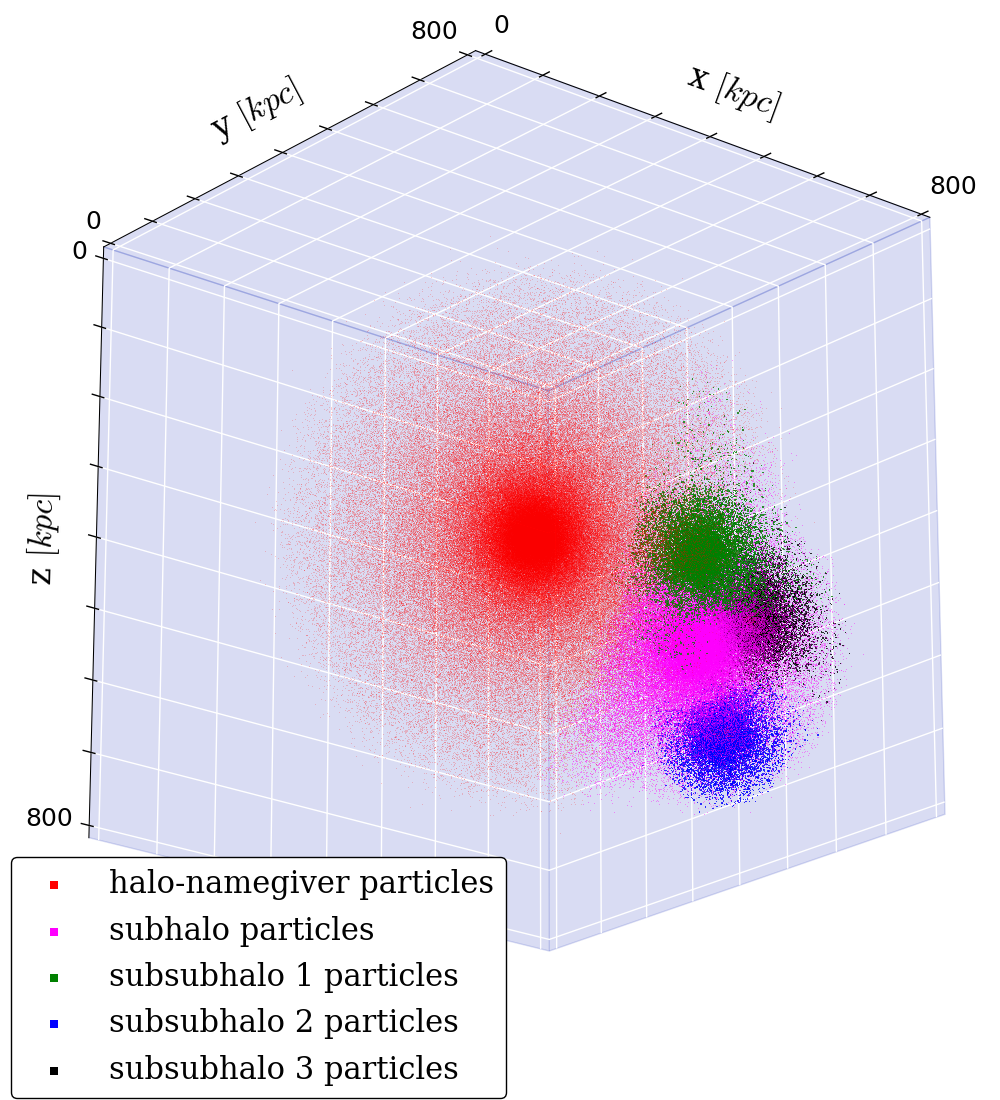
\includegraphics[width = .28\textwidth]{images/dice-sub/dice-sub-plot-halo1-nosaddle.png}} \hspace*{-1em}&
%			{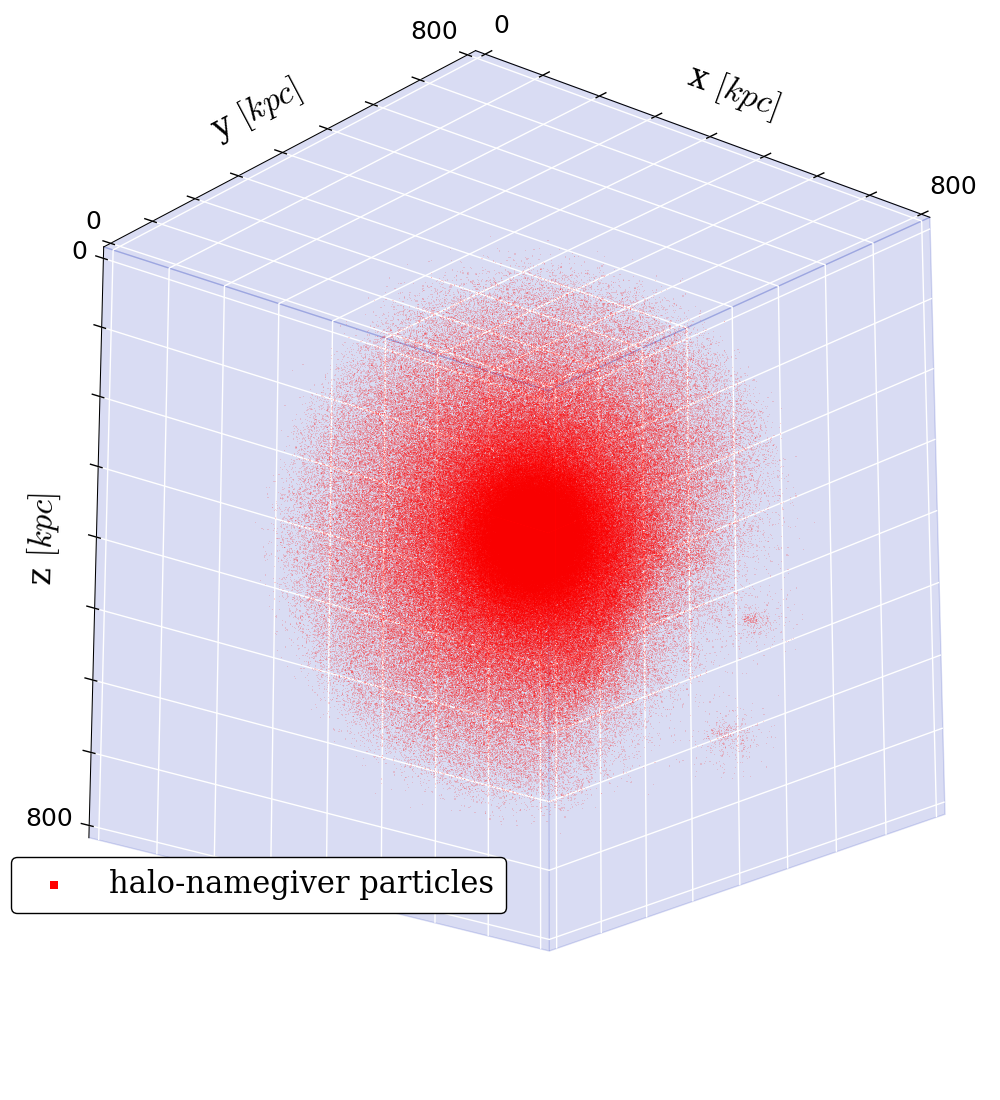
\includegraphics[width = .28\textwidth]{images/dice-sub/dice-sub-halo-only-nosaddle.png}} \hspace*{-1em}&
%			{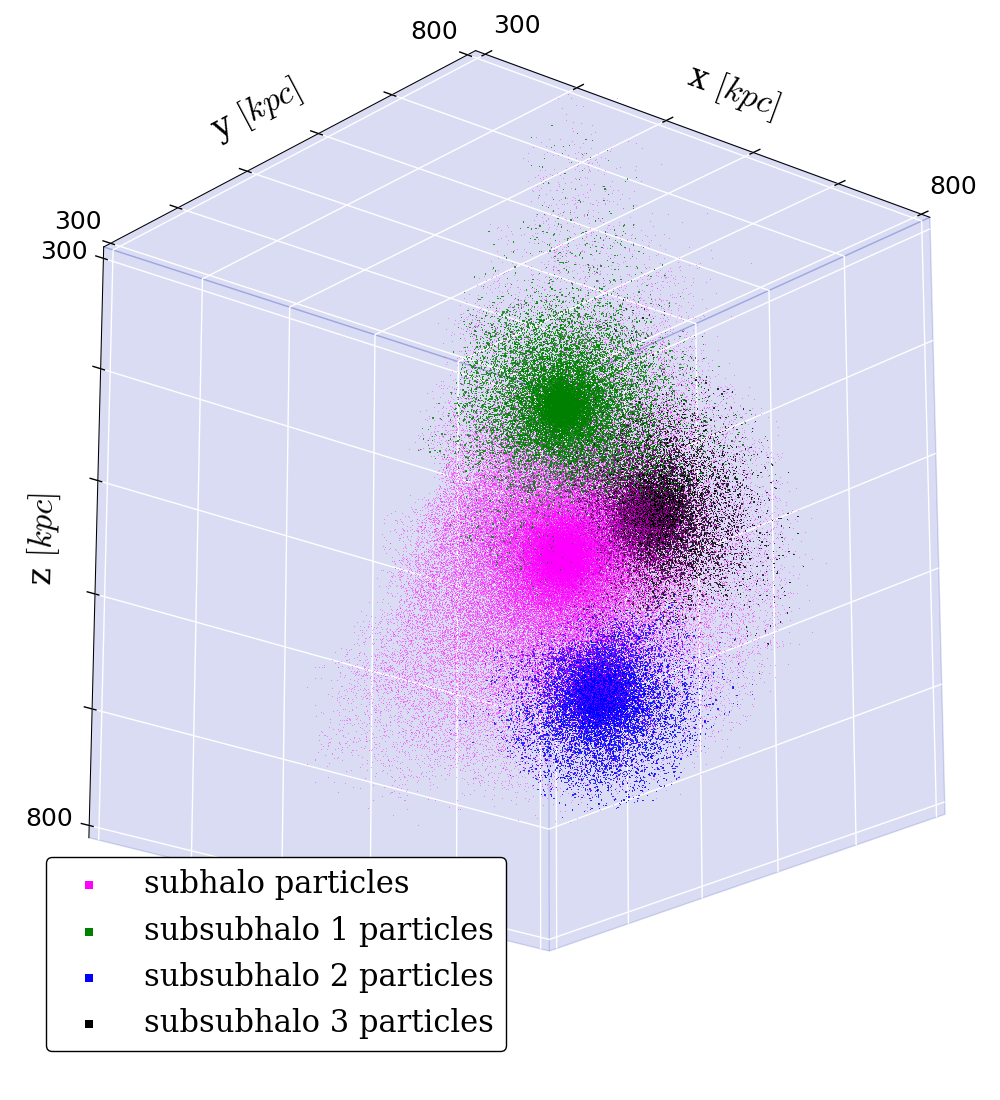
\includegraphics[width = .28\textwidth]{images/dice-sub/dice-sub-plot-subclumps-nosaddle.png}} \\
%			\hline
%		\end{tabular}
%		\label{fig:dice_sub_results_a}
%		}
%	}
%	\phantomcaption
%\end{sidewaysfigure}
%%=================================================
%%=================================================
%%=================================================
%\begin{sidewaysfigure}[!htbp]\ContinuedFloat
%	\footnotesize
%	{\renewcommand{\arraystretch}{0.1}
%	\subfloat[The results of \neigh\ and \iter\ unbinding of the \ds-dataset: All particles, halo-namegiver particles only and subclumps particles only.]{
%		\begin{tabular}{|p{1cm} c c c|}
%			\hline
%			&&&\\[1em]
%													&
%			\textbf{All particles} 					&
%			\textbf{Halo-namegiver particles only} 	&
%			\textbf{Subhalo particles only}			\\[1em]
%			%
%			%
%			\begin{sideways}{ \hspace{3cm}\neigh\ unbinding }\end{sideways}		\hspace*{-1em}		 &		
%			{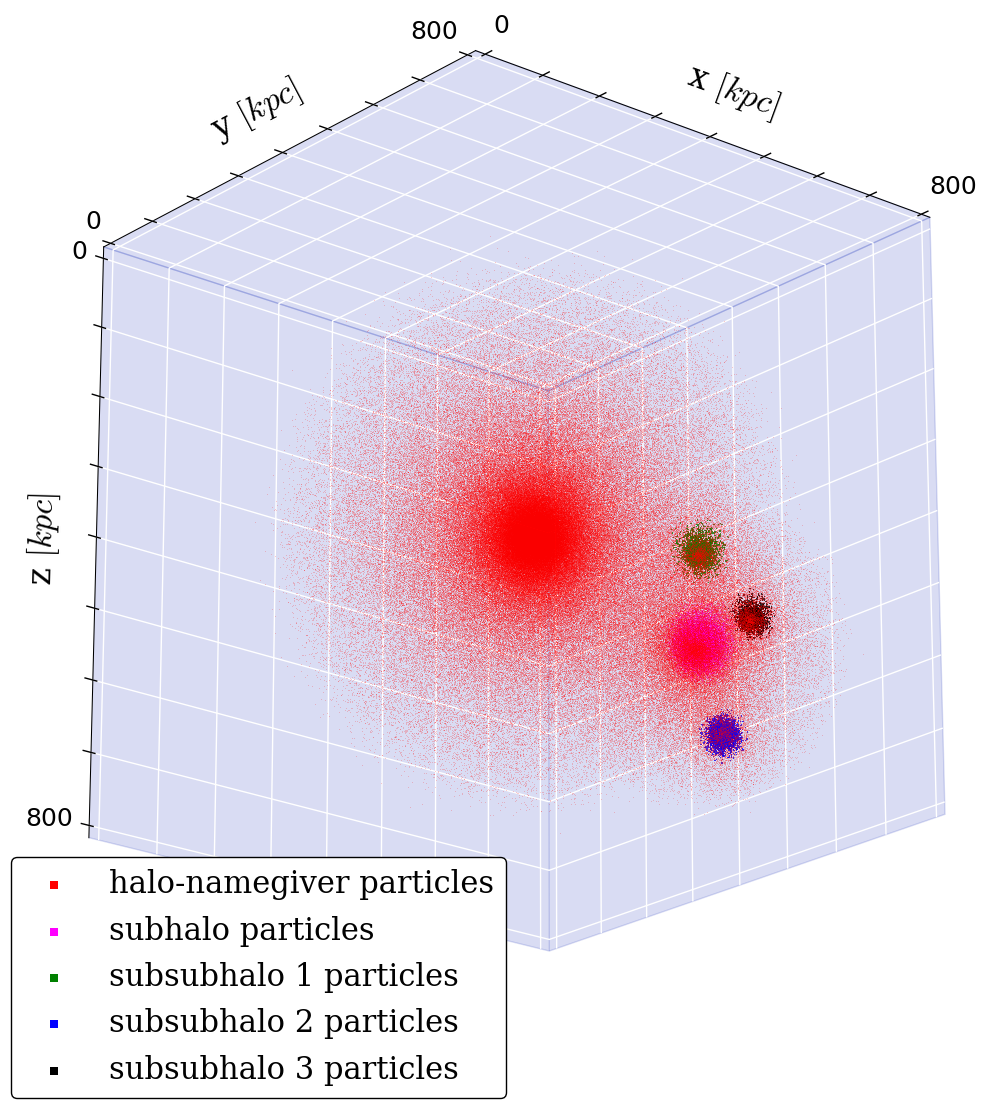
\includegraphics[width = .28\textwidth]{images/dice-sub/dice-sub-plot-halo1-saddle.png}}\hspace*{-1em} &
%			{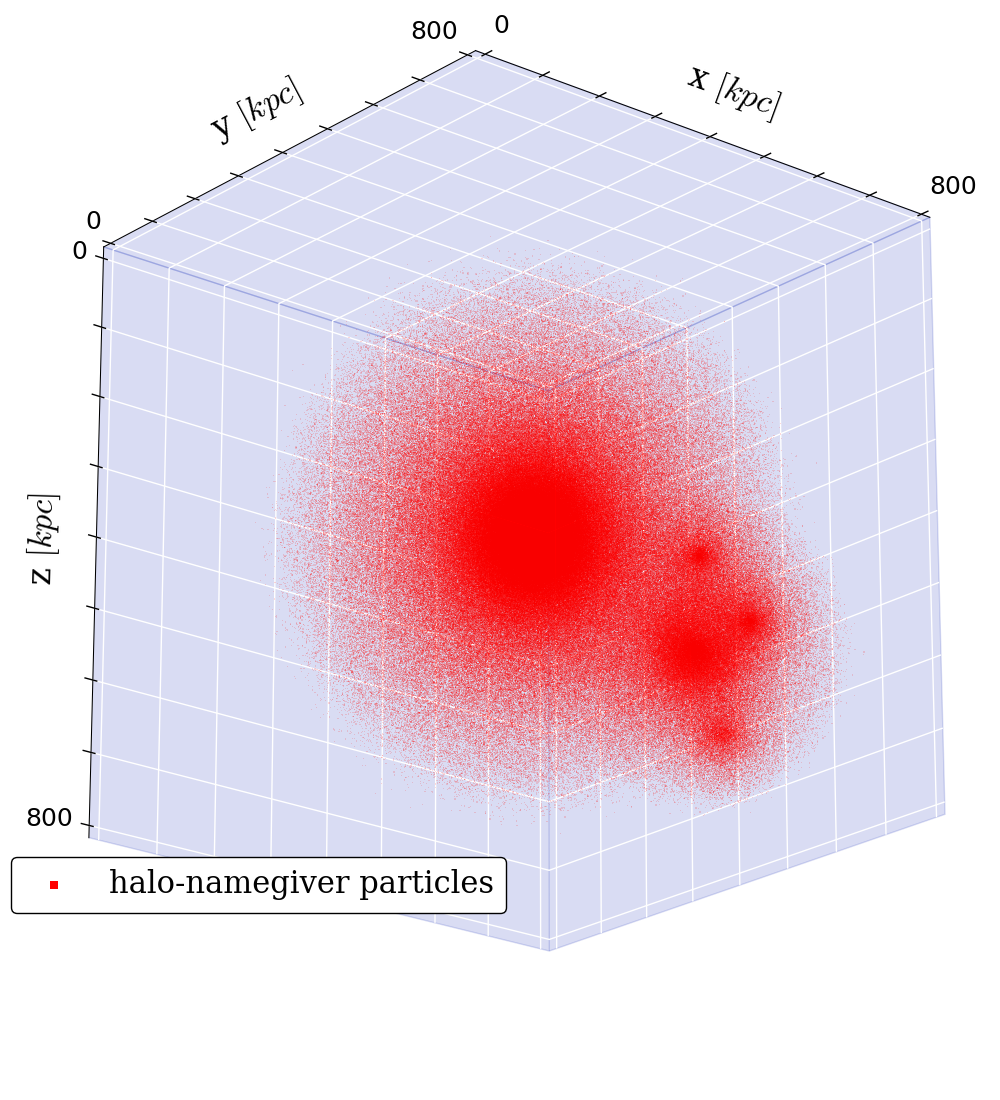
\includegraphics[width = .28\textwidth]{images/dice-sub/dice-sub-halo-only-saddle.png}}\hspace*{-1em} &
%			{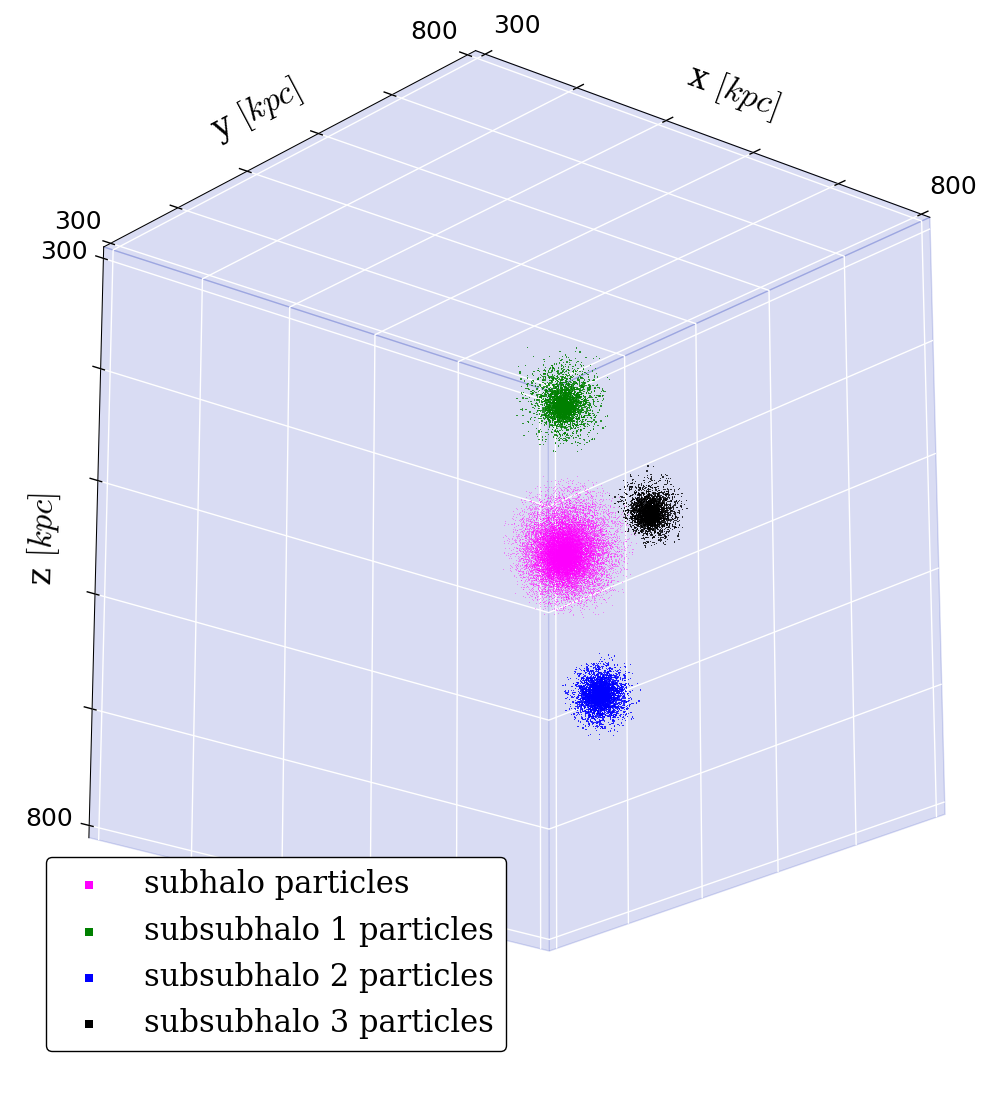
\includegraphics[width = .28\textwidth]{images/dice-sub/dice-sub-plot-subclumps-saddle.png}} \\
%	%		%
%	%		%
%			\begin{sideways}{\hspace{3cm} \iter\ unbinding }\end{sideways}		\hspace*{-1em}		 &		
%			{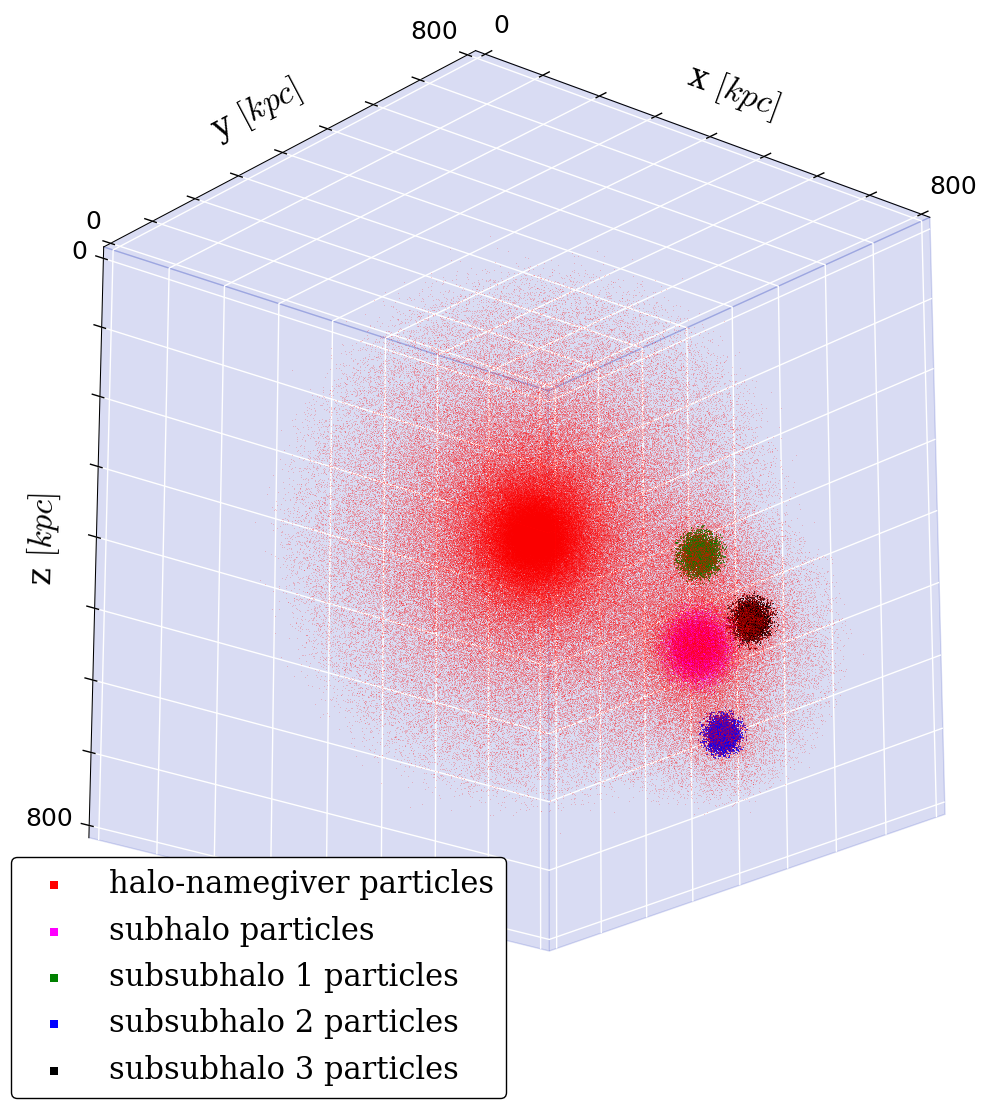
\includegraphics[width = .28\textwidth]{images/dice-sub/dice-sub-plot-halo1-iter.png}} \hspace*{-1em}&
%			{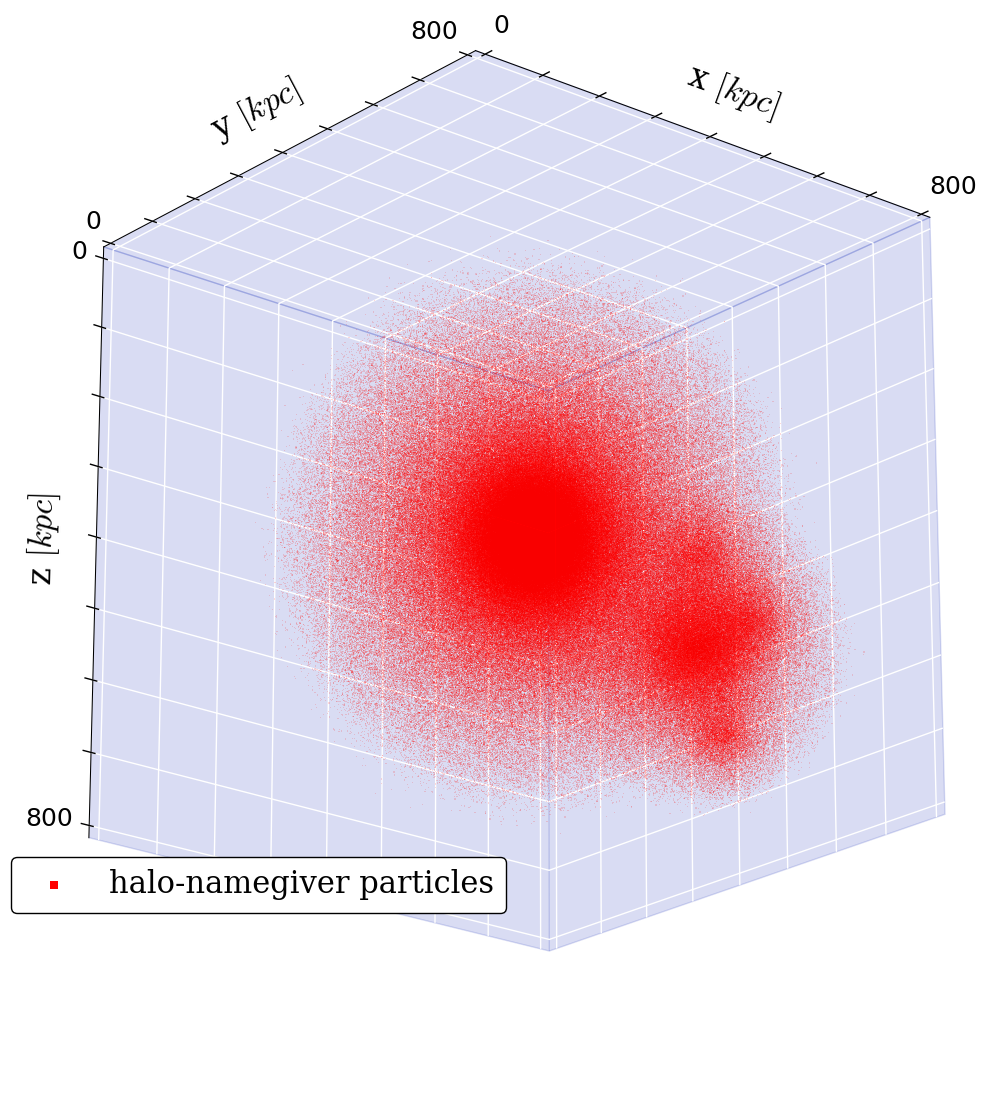
\includegraphics[width = .28\textwidth]{images/dice-sub/dice-sub-halo-only-iter.png}} \hspace*{-1em}&
%			{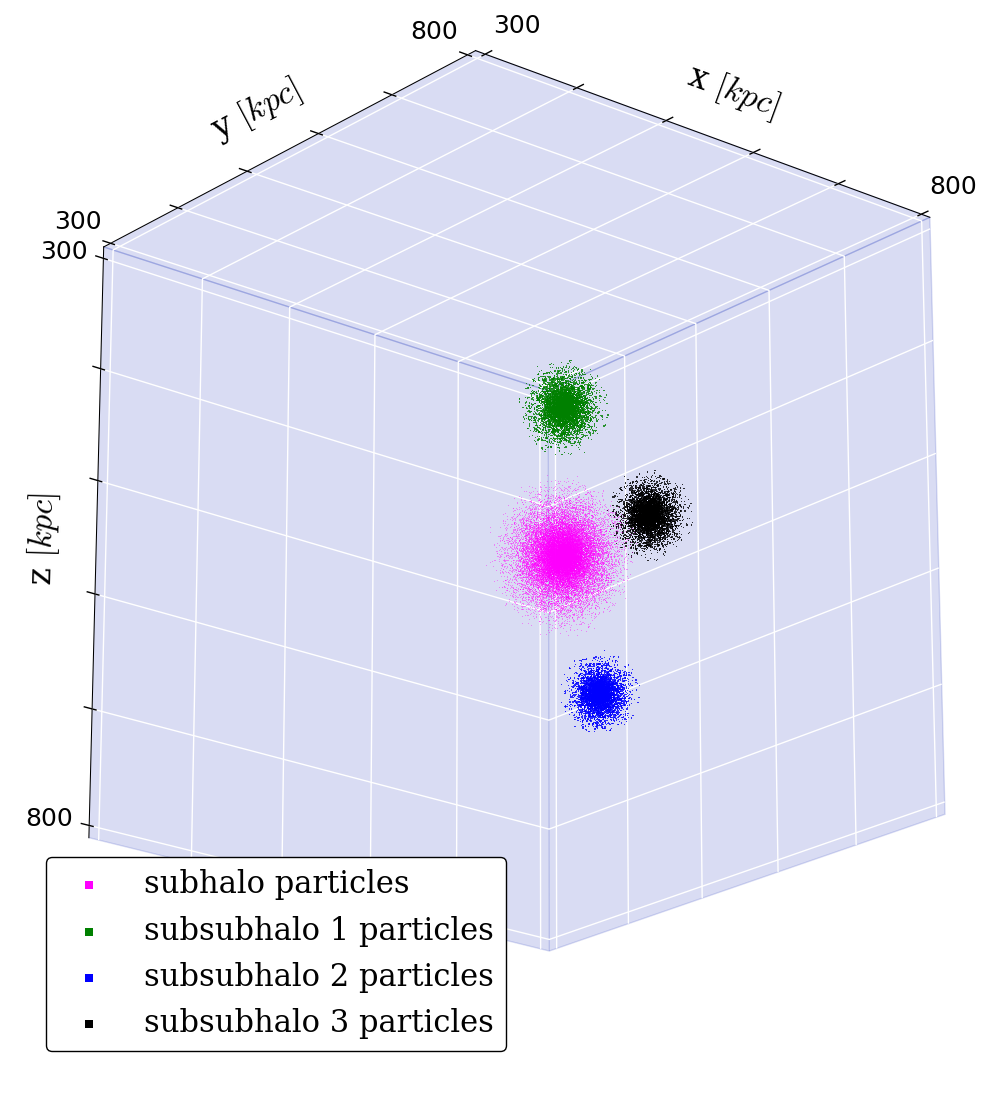
\includegraphics[width = .28\textwidth]{images/dice-sub/dice-sub-plot-subclumps-iter.png}} \\
%			%
%			%
%			\hline
%		\end{tabular}
%		\label{fig:dice_sub_results_b}
%		}
%	}
%	\caption{
%	The results of different unbinding methods on the \dt-dataset.
%	}
%	\label{fig:dice_sub_results}
%\end{sidewaysfigure}
%
%




